\documentclass[12pt,a4paper,Spanish]{book}
%Va a ser un libro (book), el tamaño es a4, la lengua castellano%%%

%\[spanish]{babel} %palabras de multitud de idiomas. Aquí no se si 
\usepackage[utf8]{inputenc} %cambio latin por utf-8
\usepackage{amsmath} %macros AM
\usepackage{amsthm} %macros AMS para teoremas.
\usepackage{amsfonts} %Permite usar fuentes.
%\usepackage[dvips]{epsfig} %Inclusión de figuras postscript
\usepackage{indentfirst}
\usepackage{graphicx}
\usepackage{subfigure}
\usepackage{hyperref}
\setlength{\parskip}{8mm} %Separación entre parrafos 
\usepackage{multirow, array} % para las tablas
%\usepackage{longtable} % para tablas largas
\usepackage{afterpage}
\usepackage[left=3 cm,top=2.5cm,right=3cm,bottom=2.5cm]{geometry} 
%\usepackage{cite} % para contraer referencias
\usepackage[utf8]{inputenc}
\usepackage[backend=biber]{biblatex}
\addbibresource{biblio.bib}
\usepackage{setspace}
\spacing{1.5}
\DeclareGraphicsExtensions{.jpg, .pdf, .png, .gif, .eps}



\begin{document}

\renewcommand{\listtablename}{Índice de tablas} 

%%PORTADA%%

\begin{titlepage}
\begin{center}


\begin{figure}
	\centering

\includegraphics[width=0.3\textwidth]{./figs/logoURJC}
\end{figure}

\begin{center}
\large
ESCUELA DE INGENIERÍA DE FUENLABRADAa

\vspace*{0.15in}
GRADO EN INGENIERÍA DE SISTEMAS AUDIOVISUALES Y MULTIMEDIA \\
\vspace*{0.6in}




{\large \bf TRABAJO FIN DE GRADO}\\
\end{center}
\vspace*{0.2in}
{\large
{TÍTULO} \\
}
\vspace*{0.3in}
\vspace*{0.3in}

\vspace*{0.1in}
\end{center}

{\large
Autor: Víctor Iglesias Cuevas  \\[0.2cm]

Tutora: Rebeca Goya Esteban \\[0.15cm]

}
\vspace*{0.1in}
\vspace*{0.1in}

\begin{center}Curso académico 2023/2024\end{center}



\end{titlepage}
%%%%%%%%%%%%%%%%%%%%%%%%%
\newpage
$\ $
\thispagestyle{empty} % para que no se numere esta pagina

%%%%%%%%%%%%%%%%%%%%%dedicatoria%%%%%%%
\chapter*{}
\pagenumbering{Roman} % para comenzar la numeracion de paginas en numeros romanos
\begin{flushright}
\textit{“bla bla" ()}

\end{flushright}
%%%%%%%%%%%%%%%%%%%%%%%%%

\chapter*{Agradecimientos} % si no queremos que añada la palabra "Capitulo"
\addcontentsline{toc}{chapter}{Agradecimientos} % si queremos que aparezca en el índice
\markboth{AGRADECIMIENTOS}{AGRADECIMIENTOS} % encabezado 

AGRADECIMIENTOS 

prueba

\chapter*{Resumen}
\addcontentsline{toc}{chapter}{Resumen} % si queremos que aparezca en e

VAS ESCRIBIENDO
\tableofcontents



\cleardoublepage
\addcontentsline{toc}{chapter}{Lista de figuras} % para que aparezca en el indice de contenidos
\listoffigures % indice de figuras

\cleardoublepage
\addcontentsline{toc}{chapter}{Lista de tablas} % para que aparezca en el indice de contenidos
\listoftables % indice de tablas



%\listoffigures
%\listoftables


\pagenumbering{arabic} % para empezar la numeración con números
\chapter{Introducción}
La música juega un rol importante en la vida de la personas, aun más en la era digital. El uso de Internet ha contribuido enormemente en el crecimiento de librerías digitales de música, y con ello, la información y metadatos disponibles de cada pista de audio.
\newline
Tradicionalmente, la clasificación de música ha estado basada en catálogos de metadatos (artista, album, título de la canción, ...) \cite{yang2011music}. Esta clasificación puede no ser suficiente para el usuario. Tener acceso a una categorización de la música en función de emociones o estados de ánimo puede ser interesante.
\newline
La relación entre música y emoción ha sido objeto de muchos debates académicos e investigaciones empíricas en muchas disciplinas diferentes donde están incluidas la filosofía, la musicología, la psicología, la biología, la antropología y la sociología. Sin embargo, no fue hasta la década de los 2000, cuando el estudio de este tema desde el punto de vista de la ingeniería comenzó a desarrollar un modelo computacional de emoción musical para la recuperación y organización de la música basada en emociones.\cite{yang2011music}
Aquí es donde entra en juego el Reconocimiento Musical de Emociones (Music Emotion Recognition). MER categoriza emociones y aplica técnicas de Machine Learning (Aprendizaje Máquina) para clasificarlas, usando diferentes características extraídas de la señal acústica de la canción \cite{yang2011music}
\section{Historia y estado actual de los sistemas MER}

Las emociones son unas 
\section{Objetivos del trabajo}
El objetivo principal del trabajo es diseñar un sistema para el reconocimiento de emociones en pistas de audio.
Los objetivos específicos que se plantean son los siguientes:

\begin{itemize}
\item Estudiar el Estado del Arte de los sistemas MER
\item Examinar técnicas de Aprendizaje Máquina (Machine Learning) para la detección de emociones
\item Usar lenguage Python para:
 	\begin{itemize}
 		\item procesar de datos del banco de datos 
 		\item desarrollar algoritmos de Machine Learning
 		\item entrenar y probar los sistemas para ajustar parámetros
 		\item evaluar las técnicas de Machine Learning según su capacidad para predecir los valores requeridos 		
 	\end{itemize}

\end{itemize}

\section{Metodología y estructura de la memoria}

Metodología:

\begin{itemize}

\item Revisión bibliográfica ...

\item Aprendizaje de ...
\item Análisis exploratorio de la base de datos...

\item ...

Estructura de la memoria:

\item En el Capítulo ...

\item ...

\item ...

\item ...

\end{itemize}

\chapter{Estado del arte}
<<<< aquí hay que meter una breve introducción de lo que aparece en el estado del arte

\section{Music Emotion Recognition}
Music Emotion Recognition (MER) es un campo de estudio que se enfoca en identificar y clasificar las emociones que la música evoca en los oyentes. Para ello, se extraen las características relevantes de las pistas de audio, se procesan, se evalúan y luego se asocian con determinadas emociones \cite{gomez2021music}
\newline
MER es una de las disciplinas de alto nivel más desafiantes en Music Information Retrieval (MIR). MIR un campo de investigación que se centra en la extracción e inferencia de características significativas de la música (a partir de la señal de audio), la clasificación de la música utilizando estas características, y el desarrollo de diferentes esquemas de búsqueda y recuperación. Tiene como objetivo poner a disposición de los individuos el vasto almacén de música del mundo \cite{schedl2014music}

\subsection{Emociones}

Los modelos teóricos de la emoción adoptados por los estudios se dividieron en cuatro clases: discretos, dimensionales, misceláneos y específicos de la música \cite{eerola2012review}. 
\newline
Uno de los más comunes usado en psicología es el modelo dimensional propuesto por Russell \cite{posner2005circumplex}. El modelo consiste en la representación de las emociones a través de dos dimensiones: valencia (agrado-desagrado) y excitación (representa el nivel de valencia). Cada emoción es una representación linea de la combinación de estas dos dimensiones

\begin{figure}[h]
	\centering
	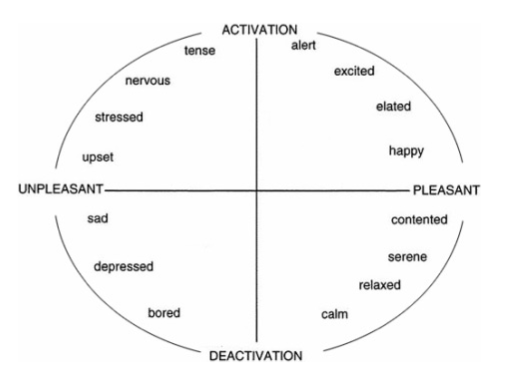
\includegraphics[width=0.7\linewidth]{figs/russell}
	\caption{Modelo dimensional de Russell}
	\label{fig:russell}
\end{figure}


Un aspecto importante en MER es la categorización de las emociones según su naturaleza. Se distinguen dos tipos:
\begin{itemize}
\item Percibidas: son aquellas que hacen referencia a las características musicales canción: tono, escala, ritmo, etc.
\item Inducidas: son las emociones que hacen referencia al contexto individual de cada persona
\end{itemize}
\cite{yang2011music} expone un ejemplo claro para distinguir entre los dos tipos: el Cumpleaños Feliz. Si analizamos la canción por sus características, se podría decir que es una canción alegre (emoción percibida). Pero es posible que para algunas personas les produzca tristeza al asociar un recuerdo con esta canción (emoción inducida)

\subsection{Estado actual MER}
\subsection{Estado futuro MER}


\section{Técnicas de Aprendizaje Máquina}

El aprendizaje máquina (Machine Learning) es la ciencia de programar ordenadores para que estos puedan aprender de los datos \cite{geron2022hands}. Se enfoca en la idea de que los ordenadores puedan "aprender" a partir de la experiencia y los datos: identifican patrones en los datos y predicen o deciden en función de esos patrones.

\subsection{Tipos de Machine Learning}
Los tipos de Machine Learning se clasifican en diferentes categorías según su naturaleza \cite{geron2022hands}:
\begin{itemize}
	\item Grado de supervisión humana durante el entrenamiento. Dentro de esta categoría se encuentran los siguientes sistemas:
	\begin{itemize}
		\item supervisados,
		\item no supervisados,
		\item refuerzo del aprendizaje (Reinforcement Learning)
	\end{itemize}
	\item Si pueden o no aprender de forma incremental. se distinguen dos tipos:
	\begin{itemize}
		\item sistemas en línea (Batch Learning),
		\item sistemas por lotes (Online Learning)
	\end{itemize}
	\item Si detectan o no patrones en los datos de entrenamiento, construyendo un modelo predictivo. Tipos:
	\begin{itemize}
		\item basados en instancias,
		\item basados en modelos
	\end{itemize}
\end{itemize}
Estos criterios no son exclusivos. Pueden combinarse de la forma que se quiera

\subsubsection{Sistemas supervisados vs. no supervisados}
Los sistemas supervisados de Machine Learning son algoritmos que utilizan datos etiquetados (etiquetas) durante la fase de entrenamiento del sistema. Son utilizados tanto para modelos de clasificación como para modelos de regresión (predicción de un número dado un paquete de características). Algunos de los algoritmos supervisados más importantes son:
\begin{itemize}
	\item KNN vecinos
	\item Regresión lineal
	\item Regresión logarítmica
	\item Redes Neuronales	
\end{itemize}
Por otro lado nos encontramos los sistemas no supervisados. Se utilizan para encontrar patrones o estructuras ocultas en datos. A diferencia de los supervisados, estos algoritmos no utilizan ningún etiquetado ni requieren de ninguna salida deseada durante el entrenamiento. Tipos de algoritmos no supervisados:
\begin{itemize}
	\item Agrupamiento (Clustering)
	\begin{itemize}
		\item K-medias
		\item DBSCAN
		\item Análisis de agrupamiento jerárquico (HCA)	
	\end{itemize}
	\item Detección de anomalías
	\begin{itemize}
		\item One-class SVM
		\item Isolation Forest	
	\end{itemize}
	\item Reducción de visualización
	\begin{itemize}
		\item Análisis de componentes principales (PCA)
		\item Kernel PCA	
		\item Locally-Linear Embedding (LLE)
		\item t-distributed Stochastic Neighbor Embedding (t-SNE)
	\end{itemize}
	\item Aprendizaje de reglas de asociación
	\begin{itemize}
		\item Apriori
		\item Eclat	
	\end{itemize}	
\end{itemize}

\subsubsection{Batch Learning y Online Learning}
Los sistemas Batch Learning son incapaces de aprender de forma incremental. El modelo se entrena utilizando la totalidad del conjunto de datos de entrenamiento de una sola vez, en lugar de hacerlo de manera incremental o en pequeñas partes. Dada la forma de entrenar, estos sistemas son capaces de captar mejor las complejidades y las variabilidades de los datos. Sin embargo, son más vulnerables frente a cambios en los datos puesto que sería necesario volver a entrenar el modelo de nuevo.
\newline
Los sistemas Online Learning son lo contrario a los anteriores: se entrenan de forma incremental. Se dividen los datos en pequeñas instancias (o mini-batches) y se alimenta el sistema de forma secuencial. Cada aprendizaje es rápido y barato. Se utiliza para sistemas donde se reciben datos de forma continua, o cuando se requiere una gran cantidad de datos para el entrenamiento. En estos modelos es importante el parámetro de tasa de aprendizaje (learning rate): Una tasa de aprendizaje alto hará que el sistema se adapte bien a cambios en los datos, pero también será más susceptible a olvidar más rápido datos antiguos


\subsubsection{Basados en instancias y Basados en modelos}
Esta clasificación hace referencia a cómo los sistemas de aprendizaje se generalizan. Por un lado están los basados en instancias: el sistema aprende los ejemplos de memoria y luego generaliza a nuevos casos comparándolos con los ejemplos aprendidos (o un subconjunto de
ellos). Es decir, utiliza una medida de similitud. Estos sistemas tiene un buen rendimiento con datos entrenados, pero no es suficiente para un sistema de Machine Learning: el verdadero objetivo es tener un buen rendimiento en instancias nuevas.
\newline
Aquí es donde se encuentran los sistemas basados en modelos, cuya forma de generalizar es a partir de modelos que hagan predicciones. Estos sistemas tienen mucho mejor rendimiento frente a instancias de datos muy ruidosas (gran cantidad de datos aleatorios). Para conseguir buenos resultados con estos sistemas se deben seguir algunos pasos como: selección del modelo (elegir el mejor modelo que se adapte a nuestro sistema), ajuste del modelo (elección correcta de los parámetro o hiperparámetros),  o entrenamiento el modelo.

\section{Modelos de Regresión}
Los modelos de Regresión son técnicas que se utilizan para predecir un valor numérico continuo basado en una o más variables independientes. Para ello, se modela el efecto de un conjunto de variables explicativas sobre una varibale de interés primario \autocite{fahrmeir2013regression}.
\newline
Los conceptos fundamentales de los modelos de Regresión son:
\begin{itemize}
	\item Variable Dependiente (variable objetivo, respuesta o de interés primario): es la variable que se desea predecir. Esta puede ser continua, binaria, categórica o de recuentos
	\item Variables explicativas: también llamadas covariables, variables independientes o regresoras. Son las que se utiliza para predecir la variable dependiente. Existen varios tipos de estas variables como continuas, binarias,	o categóricas. En modelos complejos también es posible incluir escalas temporales, variables para describir la distribución espacial o la ubicación geográfica, o indicadores grupales.
	\item Tipo de modelo: dependerá principalmente del tipo de variable respuesta, y del tipo de variables independientes
\end{itemize}
Una característica principal de los modelos de regresión es que la relación entre la variable independiente y las variables independientes no es una función determinista, si no que muestra errores. Esto implica que la respuesta \textit{y} es una variable aleatoria, cuya distribución depende de las variables independientes. Un ejemplo claro sería: sabiendo la altura de los padres no se puede predecir exactamente la altura de los hijos, solo estimar una media y el grado de dispersión. A esta desviación del valor esperado se la denomina $\epsilon$ (componente aleatorio o estocástico) (por eso es muy importante estudiar la importancia de las covariables en el valor medio de la variable objetivo). La función resultante es un modelo condicional donde los valores de \textit{y} (variable objetivo) están condicionados por las covariables ($x_1, x_2, x3, ...$) y el componente aleatorio $\epsilon$:
\begin{center}
	$y = $
	E($y|x_1, ..., x_k$) = $f(x_1, ..., x_k) + \epsilon $
\end{center}
\subsection{Árbol de regresión}


\chapter{Descripción de datos}
\chapter{Experimentos}
%------------------------------------------------------------------------------------------------
%Chapter Resultados
%------------------------------------------------------------------------------------------------
\chapter{Resultados}
\chapter{Conclusiones}

%%%%%BIBLIOGRAFÍA%%%%%%%%%%%%%%%
\chapter{Bibliografía}
\printbibliography

\end{document}
